In this section, I will trace the history of my own gender identity under the framework we established earlier. I am a phenotypic male and assigned male at birth, self-identify with \ldots~honestly, I don't know, maybe non-binary. I am comfortable with all pronouns. %The female components of my gender identity will be discussed first, followed by the male components. %This section is complementary to the core biological arguments. Moreover, we will discuss some extremely controversial topics, using myself as an example of transgender people can avoid offending others.
%\texttt{AttributeError: object 'user' has no attribute 'gender\_identity'}.

I have a strong desire to adopt a more feminine name: 娇 (\textit{Jiāo}, will be addressed as ``the feminine \textit{Jiāo}''). This character means ``cute'' or ``adorable'' and features the ``woman'' radical. It is a homophone and graphically like my legal name (骄, \textit{Jiāo}, means ``pride'', relatively neutral). I suspect my preference for the feminine \textit{Jiāo} was shaped by repeated misuse. It was frequently miswritten or mistyped as the feminine \textit{Jiāo} in my life due to the input method issue. \footnote{When typing in Chinese, we use a software called ``input method.'' It gives all possible Chinese characters based on the pinyin, and the user chooses the correct character from them. It is a common thing to choose a wrong character.} I felt ashamed and uncomfortable about it when I was in elementary and middle school, but I gradually came to like it. (\cref{fig:name})

\begin{figure}[htbp]
    \centering
    \includegraphics[width=0.8\textwidth]{figures/IDs_with_feminine_name}
    \caption{The author's name was spelt as the feminine \textit{Jiāo} by others. Left: The author's middle school name tags, with the middle one written as the feminine \textit{Jiāo}, and the top and bottom ones as the author's legal name; right: The author's border pass in Nyalam County, Xizang (Tibet), with the name spelt as the feminine \textit{Jiāo} by officers.\label{fig:name}}
\end{figure}

Another memory involves the footwear I wore in primary school, which my classmates considered ``girls' shoes.'' It was a part of our school uniform, and the colours were segregated by gender: red for girls and blue for boys, and were mandatory in school. Unfortunately, I wore the red version. Because of this, I faced physical bullying: my shoes were thrown away, my trousers were pulled down to ``check whether I was a girl,'' and I was once pushed into a bush, leading to perineal injury. At that time, I often dreamed of losing my feet, which brought me a strong sense of relief upon waking. In contrast to Body Integrity Identity Disorder, I hypothesise that I believed wearing ``girls' shoes'' rendered my feet ``girls' feet,'' prompting a desire to sever them from me to ``protect'' my ``boy'' identity.

These shoes likely originated from Japanese indoor shoes (上履き, \textit{uwabaki}), mainly used in schools and kindergartens in Japan. Chinese clothing factories might produce these shoes to export to Japan, which were later sold in China. Due to their simple style and low price, they became widely used as uniform shoes for elementary school students. \textcite{Kanzaki2019Shogakko} show that the colour of indoor shoes also usually depends on gender in Japan, but some schools assign colours by grade level. Their study revealed that the shoe itself has no fixed gender meaning; its gender meaning is artificially assigned in a specific context. (\cref{fig:shoes})

\begin{figure}[htbp]
    \centering
    \includegraphics[width=0.6\textwidth]{figures/shoes}
    \caption{Application of this kind of shoes in different contexts: a-b) Photos of the author wearing red shoes in childhood; c) A performance at a Chinese kindergarten, where boys wear the blue version and girls wear the red version, from Qilu.com; d) Screenshot from the social platform Xiaohongshu, where a Japanese blogger shares their school life, with both boys and girls wearing the red version. Chinese users in the comments discuss this phenomenon with the Japanese blogger.\label{fig:shoes}}
\end{figure}

It is also a crucial childhood memory that adults considered my ``personality was like a little girl's,'' probably because I liked playing with stuffed animal toys and disliked sports and fighting. I was punished for imitating a little girl on a TV series, covering her mouth to laugh, being told, ``Boys can't laugh like girls.'' Additionally, the boys in my class often fought. I disliked playing with them. The girls were friendly, and they were kind to me, so I enjoyed playing with them. \footnote{I am not saying that this gender-specific behaviour pattern is innate.}

%Children have no gender bias and imitate and learn all behaviours within their capabilities, and the gender meaning is externally imposed. I might have some innate personality traits and temperaments from my nervous system that are like the ``feminine temperament'' in gender stereotypes, making me more willing to imitate specific behaviours. However, these innate traits are fundamentally neutral. It has nothing to do with gender before being interpreted by adults as ``this is girls' behaviour.''

%One thing I remember vividly is when we visited a museum with an interactive exhibit. Our class was split into two groups, boys and girls. When the boys' group played, if someone failed, they were harshly mocked and heckled by the majority, telling them to get down quickly and not waste others' time. When the same thing happened in the girls' group, it was filled with encouragement. I really envied the girls' group at that moment.

I also recalled a few things related to the girls' bathroom. In elementary school, I played tag with a few girls, and they repeatedly ran into the girls' bathroom to hide. I stood at the door, waiting to catch them when they came out, but a teacher saw me and punished me. Another incident was that a maths teacher of ours punished some boys by making them clean the girls' bathroom. Additionally, I got sick and vomited during class, and the teacher took me to the girls' bathroom to clean up. These incidents are difficult to interpret with normal logic. I suspect that they shaped the girls' bathroom in my young mind into a mysteria place filled with indescribable implies and metaphors.
%it was a safe zone for girls, where they could hide during a game, while my attempt to use a logical strategy to win the game was inexplicably punished; it was a place of ``degradation'' for boys, where misbehaving boys were forced to enter and clean as a form of humiliation; it was a place of care, where when I was unwell, the usually forbidden rules were broken, and the teacher helped me clean my body and clothes. These events may have somehow shaped my fascination with female spaces, femininity, and female symbols.

One thing that left a deep impression on me was that I had a crush on a girl in my childhood, but she didn't love me. I happened to read Stefan Zweig's \textit{Letter from an Unknown Woman}, in which the female protagonist has a one-night stand with the male protagonist and raises their child on her own. I thought at the time, ``Wow, I also want to have XX's child and raise them secretly.'' It is so great that girls can have babies; it is so enviable. Why can't a boy's body have babies? What a pity. This was an envy of a specific function, stemming from a longing for a romantic relationship.

%\footnote{I know this behaviour might be considered ``shameless'' or ``perverted'' by adults, but for my kindergarten self, it was just an objective exploration of the body, which I believe is no different in essence from sucking one's thumb or playing with one's hair.}

%As we've discussed before, gender incongruence about physical characteristics and gender incongruence about social roles do not have the same neurological mechanisms. Otherwise, it would imply that humans can innately feel the traditionally defined ``gender'' (the sex-gender complex), which suggests a return to gender essentialism. Innate body incongruence may stem from the body representation. In contrast, nurture body incongruence may stem from the meaning that society and culture assign to the body and its impact on body image. Mine seems to be the latter. My dysphoria is primarily about identity and social roles \footnote{It has been explained by childhood experiences like the shoes and the girls' bathroom. }, and my longing for a female body is much milder than what other transgender people describe.

%Moreover, I find a kind of beauty in the female body that is hard to describe. It's a pre-linguistic aesthetic feeling, which could perhaps be described as ``a sense of elegance.'' I find the female body very pleasing to look at and feel envious. It's like how one might envy a bird for being able to fly, but it is unlikely to cause a body integrity disorder regarding one's own arms. \footnote{Our arms are homology with birds' wings. } I interpreted it as my longing for a female body is aesthetic and functional, not metaphysical.

%I suspect that both my so-called ``sexual orientation'' (towards women) and the aesthetic part of my ``gender identity'' are products of this aesthetic experience, combined with different ``other factors'' (to use the term loosely). Combined with intimate emotions and sexual instincts, it becomes sexual orientation; combined with body image and external stimuli, it becomes the aesthetic part of ``gender identity.''
A DeepNude version of my feminised self has sexually aroused me. In my case, ``sexual orientation'' and ``gender identity'' may share some more fundamental factors. This is phenotypically like the autogynephilia in the theory of \textcite{Blanchard1991Clinical}. However, he explained that sexual orientation is the root cause, from which gender identity stems. This implies an innate, ontological sexual orientation, which I disagree with. I believe humans have neurological aesthetic and mate preferences, but they are not innately ``gendered.'' They are interpreted by society and culture. Combined with intimate emotions and sexual instincts, it becomes sexual orientation; combined with body image and external stimuli, it becomes the aesthetic part of ``gender identity.''

I discovered the mechanism of masturbation at a very young age (around kindergarten age) and excitedly shared it with others. This indicates that my body representation was consistent with my body. However, I have neurodermatitis (also known as lichen simplex chronicus) in my scrotum. There are multiple studies supporting that chronic itching and pain can affect one's body image \parencite{Simsek2020Body, Vamos1993Body}. This could be a reason why I dislike my reproductive organs. However, it should be noted that I developed neurodermatitis much later than the childhood events mentioned above, and neurodermatitis itself is a psychosomatic disease heavily influenced by psychological and mental states \parencite{Lotti2008Prurigo, Tey2013Psychosomatic}. Therefore, it might be a result of gender dysphoria rather than a cause.

Therefore, we conclude that: my current so-called ``gender identity'' is a synthesis of this aesthetic longing for the female body, envy of the reproductive function, and an internalised reaction to childhood experiences and trauma. Our life experiences and psychological responses to external stimuli are interwoven like a dense net, or rather, like a chain reaction, where one event triggers multiple preceding events, which continue to trigger subsequent events. Then we pick out a few phenotypically similar phenomena, give them a name: ``gender identity.'' This is pure tautology and has no other meaning. (\cref{fig:bundle})

\begin{figure}[htbp]
    \centering
    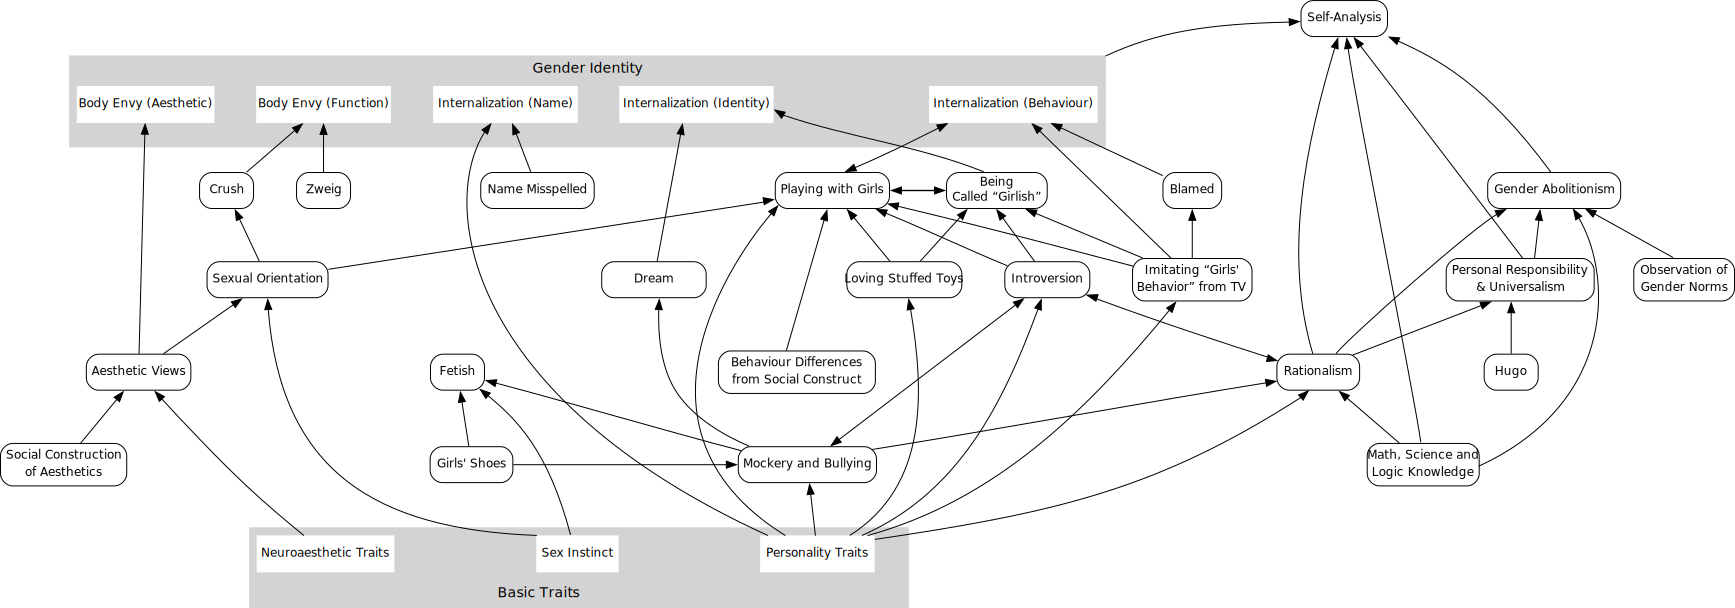
\includegraphics[width=\textwidth]{figures/bundle_of_gender_identity}
    \caption{Origins of the author's gender identity. Visualised using graphviz \parencite{Ellson2001Graphviz} and manually corrected with Inkscape \parencite{Inkscape}. Due to space and constraint limitations, the neurodermatitis and the events about girls' bathroom are not shown in the diagram.\label{fig:bundle}}
\end{figure}

The ``similarity'' and ``relatedness'' between them is also shaped by society and culture; otherwise, they would be independent and unrelated phenomena. From beginning to end, gender is not inherent in the individual (me), but in the external society. It is the pervasively gendered society and culture that assigns a gender to everything, including our bodies, clothes, behaviours and personalities. The individual, in the interaction with these ``gendered'' things, internalises social norms and develops a so-called ``gender identity.'' Therefore, ``gender identity'' is not an internal attribute but one of many components of our ``narrative identity'', it is the product of the neuroplasticity of our brains. The childhood traumas (e.g., my experience with the shoes) are also an important part that shaped our gender identities, just like they could shape other components in our narrative identities.

% Does a name have a gender? \footnote{Chinese is a language without grammatical gender. } Does a specific colour and style of shoe have a gender? Does encouragement and care from friends have a gender? Does playing with stuffed animals, disliking sports, roughhousing, or covering one's mouth to laugh have a gender? Does a specific geographical space, if not labelled ``Girls' Bathroom,'' have a gender? Does a specific body morphology and aesthetic preference have a gender? Does wanting to establish a relationship with a romantic partner through childbirth have a gender? \footnote{Some might argue that the last two do have a ``gender,'' which involves innate body representation differences. Still, we have already argued that this is a category error. Moreover, even from a biological perspective, a person can have a ``phenotypic female'' body or a uterus and simultaneously produce sperm.}

%Subsequently, I turned to another question: Is my ``gender identity'' really ``female''? This seems to be a Texas Sharpshooter Fallacy. Before I began my analysis, I had presupposed that ``I have a strong sense of identity with female identity and related social symbols.'' However, sometimes I very naturally and automatically think of myself as ``male,'' especially when arguing with trans-exclusionary radical feminists (TERFs) online.

On the other hand, the male components are relatively simple: body representation congruence and the external imposed male socialisation. In particular, there is a representative anecdote worth mentioning. I have a deep aversion to radical ``feminists'' who attack and stigmatise all men.

We learned Victor Hugo's \textit{Letter to Captain Butler on the Expedition to China} (\textit{L'Expédition de Chine. Au capitaine Butler}) in middle school language art courses:

\begin{quotation}
    However, I protest, and I thank you for giving me this opportunity. The crimes of the rulers are not the fault of the ruled; governments are sometimes bandits, but the people never are.
    \par Mais je proteste, et je vous remercie de m'en donner l'occasion; les crimes de ceux qui mènent ne sont pas la faute de ceux qui sont menés; les gouvernements sont quelquefois des bandits, les peuples jamais.
\end{quotation}

Compared to a German writer who declared in Hualing Nieh Engle's \textit{Dear Papa and Mama} (亲爱的爸爸妈妈), ``I feel as if it was I who killed those children. We are simply beasts!'', I firmly stand with Hugo's individualist morality. Although this German writer made some seemingly ``profound'' reflections, he essentially still saw himself and the Nazis as ``fellow Germans,'' sharing a transcendental guilt or sin.

When debating with radical ``feminists'', the anger is the same as I felt when debating with extreme nationalists who proclaim that ``all Japanese people are guilty, there are no innocent souls under the atomic bomb.'' \footnote{Referring to Hiroshima and Nagasaki.} They claimed my anger is because ``you're a man'' and has been ``triggered'' \footnote{急了 - jí le, a Chinese internet slang for getting flustered or angry when your weak spot is hit}, dismissed my use of literature (like the Hugo quote) as mere ``post-hoc rationalisation.'' ``You think reason is more important than the real pain and experience of women. This is a thought of male privilege. You fundamentally do not understand our female experience.''

While the truth is precisely the opposite: it is because I was arguing with them to defend my ethical principles against irrationality and collective responsibility, and in this process, I was defined as ``male,'' which shaped the male aspect of my self-identity. Thus, this phenomenon not only occurs in childhood but also appears continuously throughout a person's life. It is just that for most people, whether cisgender or transgender, after their gender identity is established, they will consciously resist the invasion from another gender. I happen to not care much about ``gender.'' I don't think my gender identity is very important to me, not my core identity, so I didn't resist it.

More importantly, my reliance on reason is not ``a thought of male privilege.'' My childhood experiences made me feel that the real world is chaotic and painful, while mathematics, logic, and science are orderly and beautiful. I remember very clearly when I was being bullied, how my heart raced, my legs trembled, and tears streamed down my face uncontrollably, while I insisted on telling them, ``You only hit me because your ideas are all unreasonable, because you can't win a debate against me.'' For me, reason has never been masculine. It is intimately intertwined with the most feminine part of my gender identity. Reason was the only shield of that little kid in the red shoes in their most vulnerable moment.

%From a particular perspective, this is also ``internalising a gender identity through interaction with a pervasively gendered society.'' TERFs use a crude, essentialist method to impose the label ``male'' on me. For the sake of debate, I strategically accept this label and develop complex emotional reactions around it. This ``contextual male identity'' and the ``female identity,'' I feel, in many other scenarios, are formed by the exact same mechanism.

%When they criticise or insult all ``phenotypic males'' in some gender-essentialist way (e.g., ``all men are oppressors''), I feel very angry and use myself as a counterexample to refute them. Of course, this is partly because I know very well that their so-called ``men'' refers to phenotypic sex, not gender identity, and I had not thought about the gender issue at that time. It at least shows that although I usually feel uncomfortable when being called or classified as ``male,'' this discomfort is not greater than my hatred for irrationality. If classifying myself as ``male'' can provide a valid counterexample to refute their argument. I am happy to substitute myself into $ \text{Male}(x) $ and logically falsify their universal proposition of $ \forall x (\text{Male}(x) \rightarrow P(x)) $.
%
%While for me personally, there is a significant difference between these two situations: I am obviously not Japanese, so when I argue with extreme nationalists, I am very clear that this is a purely rational anger against irrationality. In the other situation, because I had not deeply thought about gender identity at the time, and their definition of ``male,'' along with that of the broader society, did include me, the target and direction of this anger were often confused. I sometimes genuinely felt that I was a (specifically defined) ``male'' and that I was being insulted.
%
